% Options for packages loaded elsewhere
\PassOptionsToPackage{unicode}{hyperref}
\PassOptionsToPackage{hyphens}{url}
\PassOptionsToPackage{dvipsnames,svgnames,x11names}{xcolor}
%
\documentclass[
  letterpaper,
  DIV=11,
  numbers=noendperiod]{scrartcl}

\usepackage{amsmath,amssymb}
\usepackage{iftex}
\ifPDFTeX
  \usepackage[T1]{fontenc}
  \usepackage[utf8]{inputenc}
  \usepackage{textcomp} % provide euro and other symbols
\else % if luatex or xetex
  \usepackage{unicode-math}
  \defaultfontfeatures{Scale=MatchLowercase}
  \defaultfontfeatures[\rmfamily]{Ligatures=TeX,Scale=1}
\fi
\usepackage{lmodern}
\ifPDFTeX\else  
    % xetex/luatex font selection
\fi
% Use upquote if available, for straight quotes in verbatim environments
\IfFileExists{upquote.sty}{\usepackage{upquote}}{}
\IfFileExists{microtype.sty}{% use microtype if available
  \usepackage[]{microtype}
  \UseMicrotypeSet[protrusion]{basicmath} % disable protrusion for tt fonts
}{}
\makeatletter
\@ifundefined{KOMAClassName}{% if non-KOMA class
  \IfFileExists{parskip.sty}{%
    \usepackage{parskip}
  }{% else
    \setlength{\parindent}{0pt}
    \setlength{\parskip}{6pt plus 2pt minus 1pt}}
}{% if KOMA class
  \KOMAoptions{parskip=half}}
\makeatother
\usepackage{xcolor}
\setlength{\emergencystretch}{3em} % prevent overfull lines
\setcounter{secnumdepth}{-\maxdimen} % remove section numbering
% Make \paragraph and \subparagraph free-standing
\ifx\paragraph\undefined\else
  \let\oldparagraph\paragraph
  \renewcommand{\paragraph}[1]{\oldparagraph{#1}\mbox{}}
\fi
\ifx\subparagraph\undefined\else
  \let\oldsubparagraph\subparagraph
  \renewcommand{\subparagraph}[1]{\oldsubparagraph{#1}\mbox{}}
\fi

\usepackage{color}
\usepackage{fancyvrb}
\newcommand{\VerbBar}{|}
\newcommand{\VERB}{\Verb[commandchars=\\\{\}]}
\DefineVerbatimEnvironment{Highlighting}{Verbatim}{commandchars=\\\{\}}
% Add ',fontsize=\small' for more characters per line
\usepackage{framed}
\definecolor{shadecolor}{RGB}{241,243,245}
\newenvironment{Shaded}{\begin{snugshade}}{\end{snugshade}}
\newcommand{\AlertTok}[1]{\textcolor[rgb]{0.68,0.00,0.00}{#1}}
\newcommand{\AnnotationTok}[1]{\textcolor[rgb]{0.37,0.37,0.37}{#1}}
\newcommand{\AttributeTok}[1]{\textcolor[rgb]{0.40,0.45,0.13}{#1}}
\newcommand{\BaseNTok}[1]{\textcolor[rgb]{0.68,0.00,0.00}{#1}}
\newcommand{\BuiltInTok}[1]{\textcolor[rgb]{0.00,0.23,0.31}{#1}}
\newcommand{\CharTok}[1]{\textcolor[rgb]{0.13,0.47,0.30}{#1}}
\newcommand{\CommentTok}[1]{\textcolor[rgb]{0.37,0.37,0.37}{#1}}
\newcommand{\CommentVarTok}[1]{\textcolor[rgb]{0.37,0.37,0.37}{\textit{#1}}}
\newcommand{\ConstantTok}[1]{\textcolor[rgb]{0.56,0.35,0.01}{#1}}
\newcommand{\ControlFlowTok}[1]{\textcolor[rgb]{0.00,0.23,0.31}{#1}}
\newcommand{\DataTypeTok}[1]{\textcolor[rgb]{0.68,0.00,0.00}{#1}}
\newcommand{\DecValTok}[1]{\textcolor[rgb]{0.68,0.00,0.00}{#1}}
\newcommand{\DocumentationTok}[1]{\textcolor[rgb]{0.37,0.37,0.37}{\textit{#1}}}
\newcommand{\ErrorTok}[1]{\textcolor[rgb]{0.68,0.00,0.00}{#1}}
\newcommand{\ExtensionTok}[1]{\textcolor[rgb]{0.00,0.23,0.31}{#1}}
\newcommand{\FloatTok}[1]{\textcolor[rgb]{0.68,0.00,0.00}{#1}}
\newcommand{\FunctionTok}[1]{\textcolor[rgb]{0.28,0.35,0.67}{#1}}
\newcommand{\ImportTok}[1]{\textcolor[rgb]{0.00,0.46,0.62}{#1}}
\newcommand{\InformationTok}[1]{\textcolor[rgb]{0.37,0.37,0.37}{#1}}
\newcommand{\KeywordTok}[1]{\textcolor[rgb]{0.00,0.23,0.31}{#1}}
\newcommand{\NormalTok}[1]{\textcolor[rgb]{0.00,0.23,0.31}{#1}}
\newcommand{\OperatorTok}[1]{\textcolor[rgb]{0.37,0.37,0.37}{#1}}
\newcommand{\OtherTok}[1]{\textcolor[rgb]{0.00,0.23,0.31}{#1}}
\newcommand{\PreprocessorTok}[1]{\textcolor[rgb]{0.68,0.00,0.00}{#1}}
\newcommand{\RegionMarkerTok}[1]{\textcolor[rgb]{0.00,0.23,0.31}{#1}}
\newcommand{\SpecialCharTok}[1]{\textcolor[rgb]{0.37,0.37,0.37}{#1}}
\newcommand{\SpecialStringTok}[1]{\textcolor[rgb]{0.13,0.47,0.30}{#1}}
\newcommand{\StringTok}[1]{\textcolor[rgb]{0.13,0.47,0.30}{#1}}
\newcommand{\VariableTok}[1]{\textcolor[rgb]{0.07,0.07,0.07}{#1}}
\newcommand{\VerbatimStringTok}[1]{\textcolor[rgb]{0.13,0.47,0.30}{#1}}
\newcommand{\WarningTok}[1]{\textcolor[rgb]{0.37,0.37,0.37}{\textit{#1}}}

\providecommand{\tightlist}{%
  \setlength{\itemsep}{0pt}\setlength{\parskip}{0pt}}\usepackage{longtable,booktabs,array}
\usepackage{calc} % for calculating minipage widths
% Correct order of tables after \paragraph or \subparagraph
\usepackage{etoolbox}
\makeatletter
\patchcmd\longtable{\par}{\if@noskipsec\mbox{}\fi\par}{}{}
\makeatother
% Allow footnotes in longtable head/foot
\IfFileExists{footnotehyper.sty}{\usepackage{footnotehyper}}{\usepackage{footnote}}
\makesavenoteenv{longtable}
\usepackage{graphicx}
\makeatletter
\def\maxwidth{\ifdim\Gin@nat@width>\linewidth\linewidth\else\Gin@nat@width\fi}
\def\maxheight{\ifdim\Gin@nat@height>\textheight\textheight\else\Gin@nat@height\fi}
\makeatother
% Scale images if necessary, so that they will not overflow the page
% margins by default, and it is still possible to overwrite the defaults
% using explicit options in \includegraphics[width, height, ...]{}
\setkeys{Gin}{width=\maxwidth,height=\maxheight,keepaspectratio}
% Set default figure placement to htbp
\makeatletter
\def\fps@figure{htbp}
\makeatother

\KOMAoption{captions}{tableheading}
\makeatletter
\@ifpackageloaded{caption}{}{\usepackage{caption}}
\AtBeginDocument{%
\ifdefined\contentsname
  \renewcommand*\contentsname{Table of contents}
\else
  \newcommand\contentsname{Table of contents}
\fi
\ifdefined\listfigurename
  \renewcommand*\listfigurename{List of Figures}
\else
  \newcommand\listfigurename{List of Figures}
\fi
\ifdefined\listtablename
  \renewcommand*\listtablename{List of Tables}
\else
  \newcommand\listtablename{List of Tables}
\fi
\ifdefined\figurename
  \renewcommand*\figurename{Figure}
\else
  \newcommand\figurename{Figure}
\fi
\ifdefined\tablename
  \renewcommand*\tablename{Table}
\else
  \newcommand\tablename{Table}
\fi
}
\@ifpackageloaded{float}{}{\usepackage{float}}
\floatstyle{ruled}
\@ifundefined{c@chapter}{\newfloat{codelisting}{h}{lop}}{\newfloat{codelisting}{h}{lop}[chapter]}
\floatname{codelisting}{Listing}
\newcommand*\listoflistings{\listof{codelisting}{List of Listings}}
\makeatother
\makeatletter
\makeatother
\makeatletter
\@ifpackageloaded{caption}{}{\usepackage{caption}}
\@ifpackageloaded{subcaption}{}{\usepackage{subcaption}}
\makeatother
\ifLuaTeX
  \usepackage{selnolig}  % disable illegal ligatures
\fi
\usepackage{bookmark}

\IfFileExists{xurl.sty}{\usepackage{xurl}}{} % add URL line breaks if available
\urlstyle{same} % disable monospaced font for URLs
\hypersetup{
  pdftitle={Plan372-hw2},
  pdfauthor={Mandy Langlois},
  colorlinks=true,
  linkcolor={blue},
  filecolor={Maroon},
  citecolor={Blue},
  urlcolor={Blue},
  pdfcreator={LaTeX via pandoc}}

\title{Plan372-hw2}
\author{Mandy Langlois}
\date{}

\begin{document}
\maketitle

\begin{Shaded}
\begin{Highlighting}[]
\FunctionTok{library}\NormalTok{(tidyverse)}
\end{Highlighting}
\end{Shaded}

\begin{verbatim}
-- Attaching core tidyverse packages ------------------------ tidyverse 2.0.0 --
v dplyr     1.1.4     v readr     2.1.5
v forcats   1.0.0     v stringr   1.5.1
v ggplot2   3.5.1     v tibble    3.2.1
v lubridate 1.9.3     v tidyr     1.3.1
v purrr     1.0.2     
-- Conflicts ------------------------------------------ tidyverse_conflicts() --
x dplyr::filter() masks stats::filter()
x dplyr::lag()    masks stats::lag()
i Use the conflicted package (<http://conflicted.r-lib.org/>) to force all conflicts to become errors
\end{verbatim}

\begin{Shaded}
\begin{Highlighting}[]
\FunctionTok{library}\NormalTok{(lubridate)}
\end{Highlighting}
\end{Shaded}

\section{Load the data from the CSV.}\label{load-the-data-from-the-csv.}

\begin{Shaded}
\begin{Highlighting}[]
\NormalTok{data }\OtherTok{=} \FunctionTok{read\_csv}\NormalTok{(here}\SpecialCharTok{::}\FunctionTok{here}\NormalTok{(}\StringTok{"Fire\_incidents.csv"}\NormalTok{))}
\end{Highlighting}
\end{Shaded}

\begin{verbatim}
Rows: 229047 Columns: 20
-- Column specification --------------------------------------------------------
Delimiter: ","
chr (14): incident_number, incident_type_description, arrive_date_time, clea...
dbl  (6): X, Y, OBJECTID, incident_type, exposure, station

i Use `spec()` to retrieve the full column specification for this data.
i Specify the column types or set `show_col_types = FALSE` to quiet this message.
\end{verbatim}

\begin{Shaded}
\begin{Highlighting}[]
\FunctionTok{head}\NormalTok{(data)}
\end{Highlighting}
\end{Shaded}

\begin{verbatim}
# A tibble: 6 x 20
      X     Y OBJECTID incident_number incident_type incident_type_description 
  <dbl> <dbl>    <dbl> <chr>                   <dbl> <chr>                     
1 -78.6  35.9   474765 07-0031665                 NA NULL                      
2 -78.7  35.8   474766 08-0017918                 NA NULL                      
3 -78.6  35.8   474767 08-0032426                 NA NULL                      
4 -78.6  35.8   474768 07-0023051                444 Power line down           
5 -78.5  35.9   474769 13-0030918                150 Outside rubbish fire Other
6 -78.6  35.9   474770 14-0004846                510 Person in distress Other  
# i 14 more variables: arrive_date_time <chr>, cleared_date_time <chr>,
#   dispatch_date_time <chr>, exposure <dbl>, platoon <chr>, station <dbl>,
#   address <chr>, address2 <chr>, apt_room <chr>, GlobalID <chr>,
#   CreationDate <chr>, Creator <chr>, EditDate <chr>, Editor <chr>
\end{verbatim}

\section{Make sure the dates and times are in the right format before
any
calculations.}\label{make-sure-the-dates-and-times-are-in-the-right-format-before-any-calculations.}

\section{Calculate the response
times.}\label{calculate-the-response-times.}

\begin{Shaded}
\begin{Highlighting}[]
\NormalTok{dispatch\_date\_time }\OtherTok{=}\NormalTok{ data }\SpecialCharTok{|\textgreater{}}
  \FunctionTok{mutate}\NormalTok{(}\AttributeTok{dispatch\_date\_time =} \FunctionTok{ymd\_hms}\NormalTok{(dispatch\_date\_time), }\AttributeTok{arrive\_date\_time =} \FunctionTok{ymd\_hms}\NormalTok{(arrive\_date\_time)) }
  
  
\NormalTok{average\_response\_time }\OtherTok{=}\NormalTok{ dispatch\_date\_time }\SpecialCharTok{|\textgreater{}}
  \FunctionTok{mutate}\NormalTok{(}\AttributeTok{response\_time =}\NormalTok{ arrive\_date\_time }\SpecialCharTok{{-}}\NormalTok{ dispatch\_date\_time) }\SpecialCharTok{|\textgreater{}}
  \FunctionTok{summarize}\NormalTok{(}\AttributeTok{response\_time =} \FunctionTok{mean}\NormalTok{(response\_time, }\AttributeTok{na.rm=}\NormalTok{T)) }
 
\NormalTok{average\_response\_time}
\end{Highlighting}
\end{Shaded}

\begin{verbatim}
# A tibble: 1 x 1
  response_time
  <drtn>       
1 318.7497 secs
\end{verbatim}

\subsection{Find the average response time by
station.}\label{find-the-average-response-time-by-station.}

\begin{Shaded}
\begin{Highlighting}[]
\NormalTok{response\_by\_station }\OtherTok{=}\NormalTok{ dispatch\_date\_time }\SpecialCharTok{|\textgreater{}}
  \FunctionTok{mutate}\NormalTok{(}\AttributeTok{response\_time =}\NormalTok{ arrive\_date\_time }\SpecialCharTok{{-}}\NormalTok{ dispatch\_date\_time) }\SpecialCharTok{|\textgreater{}}
  \FunctionTok{group\_by}\NormalTok{(station) }\SpecialCharTok{|\textgreater{}}
  \FunctionTok{summarize}\NormalTok{(}\AttributeTok{response\_time =} \FunctionTok{mean}\NormalTok{(response\_time, }\AttributeTok{na.rm=}\NormalTok{T)) }

\NormalTok{highest\_response\_time }\OtherTok{=}\NormalTok{ response\_by\_station }\SpecialCharTok{|\textgreater{}}
  \FunctionTok{filter}\NormalTok{(response\_time }\SpecialCharTok{==} \FunctionTok{max}\NormalTok{(response\_time, }\AttributeTok{na.rm=}\NormalTok{T))}
  
\NormalTok{lowest\_response\_time }\OtherTok{=}\NormalTok{ response\_by\_station }\SpecialCharTok{|\textgreater{}}
  \FunctionTok{filter}\NormalTok{(response\_time }\SpecialCharTok{==} \FunctionTok{min}\NormalTok{(response\_time, }\AttributeTok{na.rm=}\NormalTok{T))}

\NormalTok{response\_by\_station }
\end{Highlighting}
\end{Shaded}

\begin{verbatim}
# A tibble: 31 x 2
   station response_time
     <dbl> <drtn>       
 1       0 450.0000 secs
 2       1 246.7053 secs
 3       2 353.0248 secs
 4       3 284.8110 secs
 5       4 326.0335 secs
 6       5 273.7687 secs
 7       6 311.8862 secs
 8       7 284.7177 secs
 9       8 333.7066 secs
10       9 291.6525 secs
# i 21 more rows
\end{verbatim}

\begin{Shaded}
\begin{Highlighting}[]
\NormalTok{highest\_response\_time}
\end{Highlighting}
\end{Shaded}

\begin{verbatim}
# A tibble: 1 x 2
  station response_time
    <dbl> <drtn>       
1      29 495.764 secs 
\end{verbatim}

\begin{Shaded}
\begin{Highlighting}[]
\NormalTok{lowest\_response\_time}
\end{Highlighting}
\end{Shaded}

\begin{verbatim}
# A tibble: 1 x 2
  station response_time
    <dbl> <drtn>       
1      13 223 secs     
\end{verbatim}

\section{finding the station with the highest and lowest average
response over
time.}\label{finding-the-station-with-the-highest-and-lowest-average-response-over-time.}

\begin{Shaded}
\begin{Highlighting}[]
\NormalTok{response\_over\_time }\OtherTok{=}\NormalTok{ data }\SpecialCharTok{|\textgreater{}}
  \FunctionTok{mutate}\NormalTok{(}\AttributeTok{dispatch\_date\_time =} \FunctionTok{ymd\_hms}\NormalTok{(dispatch\_date\_time), }\AttributeTok{arrive\_date\_time =} \FunctionTok{ymd\_hms}\NormalTok{(arrive\_date\_time))}

\NormalTok{response\_over\_time }\OtherTok{=}\NormalTok{ response\_over\_time }\SpecialCharTok{|\textgreater{}}
  \FunctionTok{mutate}\NormalTok{(}\AttributeTok{response\_time =}\NormalTok{ arrive\_date\_time }\SpecialCharTok{{-}}\NormalTok{ dispatch\_date\_time)}

\NormalTok{response\_over\_time }\OtherTok{=}\NormalTok{ response\_over\_time }\SpecialCharTok{|\textgreater{}}
  \FunctionTok{mutate}\NormalTok{(}\AttributeTok{year =} \FunctionTok{year}\NormalTok{(dispatch\_date\_time))}

\NormalTok{response\_by\_year }\OtherTok{=}\NormalTok{ response\_over\_time }\SpecialCharTok{|\textgreater{}}
  \FunctionTok{group\_by}\NormalTok{(year) }\SpecialCharTok{|\textgreater{}}
  \FunctionTok{summarize}\NormalTok{(}\AttributeTok{response\_time =} \FunctionTok{mean}\NormalTok{(response\_time, }\AttributeTok{na.rm=}\NormalTok{T ))}

\NormalTok{response\_by\_year}
\end{Highlighting}
\end{Shaded}

\begin{verbatim}
# A tibble: 17 x 2
    year response_time
   <dbl> <drtn>       
 1  2007 310.7516 secs
 2  2008 316.6669 secs
 3  2009 286.9414 secs
 4  2010 293.6406 secs
 5  2011 297.9799 secs
 6  2012 317.3400 secs
 7  2013 314.6415 secs
 8  2014 313.8668 secs
 9  2015 302.1926 secs
10  2016 323.5524 secs
11  2017 301.9666 secs
12  2018 304.3143 secs
13  2019 420.6703 secs
14  2020 344.3216 secs
15  2021 322.6979 secs
16  2022 260.8378 secs
17    NA      NaN secs
\end{verbatim}

\begin{Shaded}
\begin{Highlighting}[]
\FunctionTok{ggplot}\NormalTok{(response\_by\_year, }\FunctionTok{aes}\NormalTok{(}\AttributeTok{x=}\NormalTok{year, }\AttributeTok{y=}\NormalTok{response\_time)) }\SpecialCharTok{+}
  \FunctionTok{geom\_line}\NormalTok{() }
\end{Highlighting}
\end{Shaded}

\begin{verbatim}
Don't know how to automatically pick scale for object of type <difftime>.
Defaulting to continuous.
\end{verbatim}

\begin{verbatim}
Warning: Removed 1 row containing missing values or values outside the scale range
(`geom_line()`).
\end{verbatim}

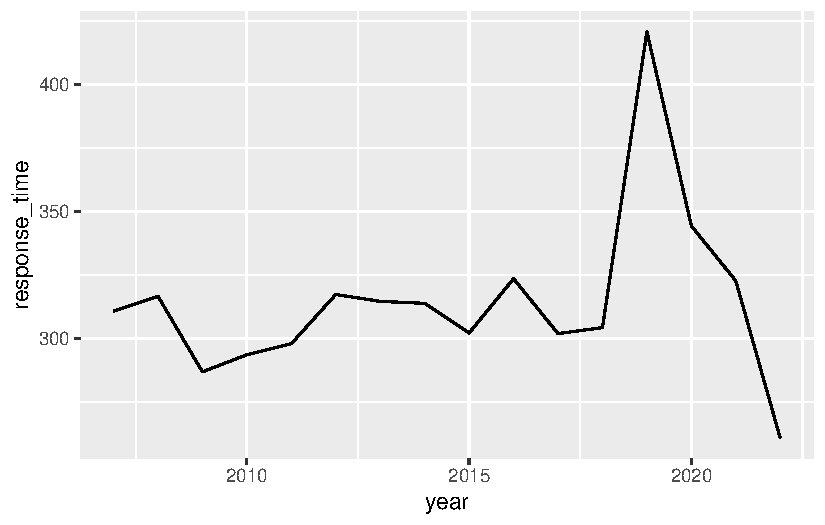
\includegraphics{hw2_files/figure-pdf/unnamed-chunk-6-1.pdf}

\section{Calculating the times of day fire calls are most likely to
occur.}\label{calculating-the-times-of-day-fire-calls-are-most-likely-to-occur.}

\begin{Shaded}
\begin{Highlighting}[]
\NormalTok{fire\_calls\_by\_time }\OtherTok{=}\NormalTok{ data }\SpecialCharTok{|\textgreater{}}
  \FunctionTok{mutate}\NormalTok{(}\AttributeTok{dispatch\_date\_time =} \FunctionTok{ymd\_hms}\NormalTok{(dispatch\_date\_time))}

\NormalTok{fire\_calls\_by\_time }\OtherTok{=}\NormalTok{ fire\_calls\_by\_time }\SpecialCharTok{|\textgreater{}}
  \FunctionTok{mutate}\NormalTok{(}\AttributeTok{hour =} \FunctionTok{hour}\NormalTok{(dispatch\_date\_time))}

\NormalTok{calls\_by\_hour }\OtherTok{=}\NormalTok{ fire\_calls\_by\_time }\SpecialCharTok{|\textgreater{}}
\FunctionTok{group\_by}\NormalTok{(hour) }\SpecialCharTok{|\textgreater{}}
  \FunctionTok{summarize}\NormalTok{(}\AttributeTok{call\_count =} \FunctionTok{length}\NormalTok{(dispatch\_date\_time)) }

\NormalTok{calls\_by\_hour}
\end{Highlighting}
\end{Shaded}

\begin{verbatim}
# A tibble: 25 x 2
    hour call_count
   <int>      <int>
 1     0      11714
 2     1      10512
 3     2       9340
 4     3       8366
 5     4       7449
 6     5       6337
 7     6       5785
 8     7       5065
 9     8       4640
10     9       4303
# i 15 more rows
\end{verbatim}

\begin{Shaded}
\begin{Highlighting}[]
\FunctionTok{ggplot}\NormalTok{(calls\_by\_hour, }\FunctionTok{aes}\NormalTok{(}\AttributeTok{x=}\NormalTok{hour, }\AttributeTok{y=}\NormalTok{call\_count)) }\SpecialCharTok{+}
  \FunctionTok{geom\_col}\NormalTok{()}
\end{Highlighting}
\end{Shaded}

\begin{verbatim}
Warning: Removed 1 row containing missing values or values outside the scale range
(`geom_col()`).
\end{verbatim}

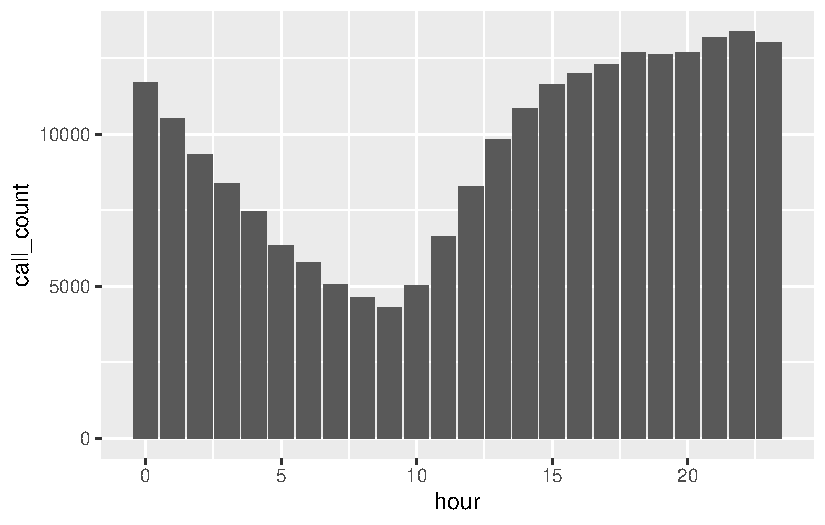
\includegraphics{hw2_files/figure-pdf/unnamed-chunk-7-1.pdf}

\section{Calculating how many calls are recorded in this
dataset.}\label{calculating-how-many-calls-are-recorded-in-this-dataset.}

\section{figure out how many of them are actual
fires.}\label{figure-out-how-many-of-them-are-actual-fires.}

\begin{Shaded}
\begin{Highlighting}[]
\NormalTok{fire\_calls }\OtherTok{=}\NormalTok{ data }\SpecialCharTok{|\textgreater{}}
  \FunctionTok{filter}\NormalTok{(incident\_type }\SpecialCharTok{\textgreater{}=} \DecValTok{100}\NormalTok{, incident\_type }\SpecialCharTok{\textless{}} \DecValTok{200}\NormalTok{)}

\NormalTok{total\_fire\_calls }\OtherTok{=} \FunctionTok{length}\NormalTok{(data}\SpecialCharTok{$}\NormalTok{incident\_type)}

\NormalTok{actual\_fires }\OtherTok{=} \FunctionTok{sum}\NormalTok{(}\SpecialCharTok{!}\FunctionTok{is.na}\NormalTok{(fire\_calls}\SpecialCharTok{$}\NormalTok{incident\_type))}

\NormalTok{total\_fire\_calls}
\end{Highlighting}
\end{Shaded}

\begin{verbatim}
[1] 229047
\end{verbatim}

\begin{Shaded}
\begin{Highlighting}[]
\NormalTok{actual\_fires}
\end{Highlighting}
\end{Shaded}

\begin{verbatim}
[1] 17231
\end{verbatim}

\section{Determine the average response time to actual
fires.}\label{determine-the-average-response-time-to-actual-fires.}

\section{Determine if the response time is faster than the average
response time for all
incidents.}\label{determine-if-the-response-time-is-faster-than-the-average-response-time-for-all-incidents.}

\begin{Shaded}
\begin{Highlighting}[]
\NormalTok{dispatch\_date\_time\_fires }\OtherTok{=}\NormalTok{ data }\SpecialCharTok{|\textgreater{}}
   \FunctionTok{filter}\NormalTok{(incident\_type }\SpecialCharTok{\textgreater{}=} \DecValTok{100}\NormalTok{, incident\_type }\SpecialCharTok{\textless{}} \DecValTok{200}\NormalTok{) }\SpecialCharTok{|\textgreater{}}
   \FunctionTok{mutate}\NormalTok{(}\AttributeTok{dispatch\_date\_time =} \FunctionTok{ymd\_hms}\NormalTok{(dispatch\_date\_time), }\AttributeTok{arrive\_date\_time =} \FunctionTok{ymd\_hms}\NormalTok{(arrive\_date\_time)) }
  
  
\NormalTok{average\_response\_time\_fires }\OtherTok{=}\NormalTok{ dispatch\_date\_time\_fires }\SpecialCharTok{|\textgreater{}}
  \FunctionTok{mutate}\NormalTok{(}\AttributeTok{response\_time =}\NormalTok{ arrive\_date\_time }\SpecialCharTok{{-}}\NormalTok{ dispatch\_date\_time) }\SpecialCharTok{|\textgreater{}}
  \FunctionTok{summarize}\NormalTok{(}\AttributeTok{average\_response\_time\_fires =} \FunctionTok{mean}\NormalTok{(response\_time, }\AttributeTok{na.rm=}\NormalTok{T)) }

\NormalTok{dispatch\_date\_time\_all }\OtherTok{=}\NormalTok{ data }\SpecialCharTok{|\textgreater{}}
   \FunctionTok{mutate}\NormalTok{(}\AttributeTok{dispatch\_date\_time =} \FunctionTok{ymd\_hms}\NormalTok{(dispatch\_date\_time), }\AttributeTok{arrive\_date\_time =} \FunctionTok{ymd\_hms}\NormalTok{(arrive\_date\_time)) }\SpecialCharTok{|\textgreater{}}
  \FunctionTok{filter}\NormalTok{(}\SpecialCharTok{!}\FunctionTok{is.na}\NormalTok{(dispatch\_date\_time), }\SpecialCharTok{!}\FunctionTok{is.na}\NormalTok{(arrive\_date\_time)) }
  
\NormalTok{  average\_response\_time\_all }\OtherTok{=}\NormalTok{ dispatch\_date\_time\_all }\SpecialCharTok{|\textgreater{}}
    \FunctionTok{mutate}\NormalTok{(}\AttributeTok{response\_time =}\NormalTok{ arrive\_date\_time }\SpecialCharTok{{-}}\NormalTok{ dispatch\_date\_time) }\SpecialCharTok{|\textgreater{}}
    \FunctionTok{summarize}\NormalTok{(}\AttributeTok{average\_response\_time\_all =} \FunctionTok{mean}\NormalTok{(response\_time, }\AttributeTok{na.rm=}\NormalTok{T))}
  
\NormalTok{  average\_response\_time\_fires}
\end{Highlighting}
\end{Shaded}

\begin{verbatim}
# A tibble: 1 x 1
  average_response_time_fires
  <drtn>                     
1 310.9837 secs              
\end{verbatim}

\begin{Shaded}
\begin{Highlighting}[]
\NormalTok{  average\_response\_time\_all}
\end{Highlighting}
\end{Shaded}

\begin{verbatim}
# A tibble: 1 x 1
  average_response_time_all
  <drtn>                   
1 318.7497 secs            
\end{verbatim}

\section{Calculating response time by station for actual
fires.}\label{calculating-response-time-by-station-for-actual-fires.}

\section{Determine which station have the highest and lowest average
response time for actual
fires.}\label{determine-which-station-have-the-highest-and-lowest-average-response-time-for-actual-fires.}

\begin{Shaded}
\begin{Highlighting}[]
\NormalTok{dispatch\_date\_time\_fires }\OtherTok{=}\NormalTok{ data }\SpecialCharTok{|\textgreater{}}
  \FunctionTok{filter}\NormalTok{(incident\_type }\SpecialCharTok{\textgreater{}=} \DecValTok{100}\NormalTok{, incident\_type }\SpecialCharTok{\textless{}} \DecValTok{200}\NormalTok{) }\SpecialCharTok{|\textgreater{}}
  \FunctionTok{mutate}\NormalTok{(}\AttributeTok{dispatch\_date\_time =} \FunctionTok{ymd\_hms}\NormalTok{(dispatch\_date\_time), }\AttributeTok{arrive\_date\_time =} \FunctionTok{ymd\_hms}\NormalTok{(arrive\_date\_time)) }\SpecialCharTok{|\textgreater{}}
  \FunctionTok{filter}\NormalTok{(}\SpecialCharTok{!}\FunctionTok{is.na}\NormalTok{(dispatch\_date\_time), }\SpecialCharTok{!}\FunctionTok{is.na}\NormalTok{(arrive\_date\_time)) }\SpecialCharTok{|\textgreater{}}
  \FunctionTok{mutate}\NormalTok{(}\AttributeTok{response\_time =}\NormalTok{ arrive\_date\_time }\SpecialCharTok{{-}}\NormalTok{ dispatch\_date\_time) }
  
\NormalTok{average\_response\_time\_by\_station\_fires }\OtherTok{=}\NormalTok{ dispatch\_date\_time\_fires }\SpecialCharTok{|\textgreater{}}
    \FunctionTok{group\_by}\NormalTok{(station) }\SpecialCharTok{|\textgreater{}}
    \FunctionTok{summarize}\NormalTok{(}\AttributeTok{average\_response\_time =} \FunctionTok{mean}\NormalTok{(response\_time, }\AttributeTok{na.rm=}\NormalTok{T))}
  
\NormalTok{highest\_response\_time\_station\_fires }\OtherTok{=}\NormalTok{ average\_response\_time\_by\_station\_fires }\SpecialCharTok{|\textgreater{}}
  \FunctionTok{filter}\NormalTok{(average\_response\_time }\SpecialCharTok{==} \FunctionTok{max}\NormalTok{(average\_response\_time, }\AttributeTok{na.rm=}\NormalTok{T))}
  
\NormalTok{lowest\_response\_time\_station\_fires }\OtherTok{=}\NormalTok{ average\_response\_time\_by\_station\_fires }\SpecialCharTok{|\textgreater{}}
  \FunctionTok{filter}\NormalTok{(average\_response\_time }\SpecialCharTok{==} \FunctionTok{min}\NormalTok{(average\_response\_time, }\AttributeTok{na.rm=}\NormalTok{T))}

\NormalTok{average\_response\_time\_by\_station\_fires}
\end{Highlighting}
\end{Shaded}

\begin{verbatim}
# A tibble: 29 x 2
   station average_response_time
     <dbl> <drtn>               
 1       1 250.0814 secs        
 2       2 439.1138 secs        
 3       3 232.7666 secs        
 4       4 276.9760 secs        
 5       5 271.0142 secs        
 6       6 289.4477 secs        
 7       7 240.8027 secs        
 8       8 295.1253 secs        
 9       9 446.2697 secs        
10      10 278.3915 secs        
# i 19 more rows
\end{verbatim}

\begin{Shaded}
\begin{Highlighting}[]
\NormalTok{highest\_response\_time\_station\_fires}
\end{Highlighting}
\end{Shaded}

\begin{verbatim}
# A tibble: 1 x 2
  station average_response_time
    <dbl> <drtn>               
1      23 586.3713 secs        
\end{verbatim}

\begin{Shaded}
\begin{Highlighting}[]
\NormalTok{lowest\_response\_time\_station\_fires}
\end{Highlighting}
\end{Shaded}

\begin{verbatim}
# A tibble: 1 x 2
  station average_response_time
    <dbl> <drtn>               
1       3 232.7666 secs        
\end{verbatim}

\section{Determine if wake forest county fire response times have been
going up or down for actual
fires.}\label{determine-if-wake-forest-county-fire-response-times-have-been-going-up-or-down-for-actual-fires.}

\section{determine the reason behind the
changes.}\label{determine-the-reason-behind-the-changes.}

\begin{Shaded}
\begin{Highlighting}[]
\NormalTok{dispatch\_date\_time }\OtherTok{=}\NormalTok{ data }\SpecialCharTok{|\textgreater{}}
  \FunctionTok{filter}\NormalTok{(incident\_type }\SpecialCharTok{\textgreater{}=} \DecValTok{100}\NormalTok{, incident\_type }\SpecialCharTok{\textless{}} \DecValTok{200}\NormalTok{) }\SpecialCharTok{|\textgreater{}}
  \FunctionTok{mutate}\NormalTok{(}\AttributeTok{dispatch\_date\_time =} \FunctionTok{ymd\_hms}\NormalTok{(dispatch\_date\_time), }\AttributeTok{arrive\_date\_time =} \FunctionTok{ymd\_hms}\NormalTok{(arrive\_date\_time)) }\SpecialCharTok{|\textgreater{}}
  \FunctionTok{filter}\NormalTok{(}\SpecialCharTok{!}\FunctionTok{is.na}\NormalTok{(dispatch\_date\_time),}\SpecialCharTok{!}\FunctionTok{is.na}\NormalTok{(arrive\_date\_time)) }\SpecialCharTok{|\textgreater{}}
  \FunctionTok{mutate}\NormalTok{(}\AttributeTok{response\_time =}\NormalTok{ arrive\_date\_time }\SpecialCharTok{{-}}\NormalTok{ dispatch\_date\_time) }
  
\NormalTok{dispatch\_date\_time\_fires }\OtherTok{=}\NormalTok{ dispatch\_date\_time\_fires }\SpecialCharTok{|\textgreater{}}
  \FunctionTok{mutate}\NormalTok{(}\AttributeTok{year =} \FunctionTok{year}\NormalTok{(dispatch\_date\_time))}

\NormalTok{average\_response\_time\_by\_year }\OtherTok{=}\NormalTok{ dispatch\_date\_time\_fires }\SpecialCharTok{|\textgreater{}}
  \FunctionTok{group\_by}\NormalTok{(year) }\SpecialCharTok{|\textgreater{}}
  \FunctionTok{summarize}\NormalTok{(}\AttributeTok{average\_response\_time =} \FunctionTok{mean}\NormalTok{(response\_time, }\AttributeTok{na.rm=}\NormalTok{T))}
  
\NormalTok{average\_response\_time\_by\_year}
\end{Highlighting}
\end{Shaded}

\begin{verbatim}
# A tibble: 15 x 2
    year average_response_time
   <dbl> <drtn>               
 1  2007 296.8353 secs        
 2  2008 334.9061 secs        
 3  2009 418.2293 secs        
 4  2010 285.1706 secs        
 5  2011 277.5476 secs        
 6  2012 296.1646 secs        
 7  2013 293.6396 secs        
 8  2014 382.4182 secs        
 9  2015 294.1111 secs        
10  2016 298.6482 secs        
11  2017 268.1704 secs        
12  2018 280.6117 secs        
13  2019 360.3776 secs        
14  2020 298.4371 secs        
15  2021 268.3878 secs        
\end{verbatim}

\begin{Shaded}
\begin{Highlighting}[]
\FunctionTok{ggplot}\NormalTok{(average\_response\_time\_by\_year, }\FunctionTok{aes}\NormalTok{(}\AttributeTok{x=}\NormalTok{year, }\AttributeTok{y=}\NormalTok{average\_response\_time)) }\SpecialCharTok{+}
  \FunctionTok{geom\_line}\NormalTok{() }
\end{Highlighting}
\end{Shaded}

\begin{verbatim}
Don't know how to automatically pick scale for object of type <difftime>.
Defaulting to continuous.
\end{verbatim}

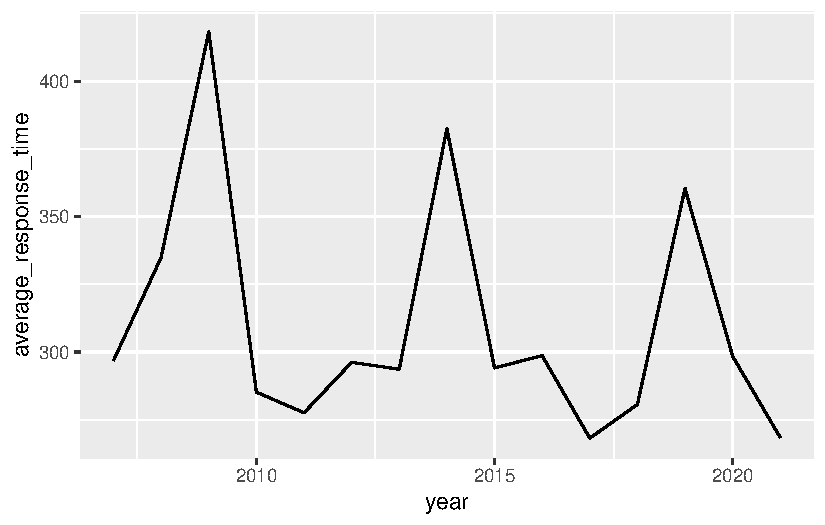
\includegraphics{hw2_files/figure-pdf/unnamed-chunk-11-1.pdf}

\section{Determine what times of day are fire calls most likely
occur.}\label{determine-what-times-of-day-are-fire-calls-most-likely-occur.}

\begin{Shaded}
\begin{Highlighting}[]
\NormalTok{fire\_calls }\OtherTok{=}\NormalTok{ data }\SpecialCharTok{|\textgreater{}}
  \FunctionTok{filter}\NormalTok{(incident\_type }\SpecialCharTok{\textgreater{}=} \DecValTok{100}\NormalTok{, incident\_type }\SpecialCharTok{\textless{}} \DecValTok{200}\NormalTok{) }\SpecialCharTok{|\textgreater{}}
  \FunctionTok{mutate}\NormalTok{(}\AttributeTok{dispatch\_date\_time =} \FunctionTok{ymd\_hms}\NormalTok{(dispatch\_date\_time))}

\NormalTok{fire\_calls }\OtherTok{=}\NormalTok{ fire\_calls }\SpecialCharTok{|\textgreater{}}
  \FunctionTok{mutate}\NormalTok{(}\AttributeTok{hour =} \FunctionTok{hour}\NormalTok{(dispatch\_date\_time))}

\NormalTok{calls\_by\_hour }\OtherTok{=}\NormalTok{ fire\_calls }\SpecialCharTok{|\textgreater{}}
  \FunctionTok{group\_by}\NormalTok{(hour) }\SpecialCharTok{|\textgreater{}}
  \FunctionTok{summarize}\NormalTok{(}\AttributeTok{call\_count =} \FunctionTok{length}\NormalTok{(dispatch\_date\_time))}

\NormalTok{calls\_by\_hour}
\end{Highlighting}
\end{Shaded}

\begin{verbatim}
# A tibble: 25 x 2
    hour call_count
   <int>      <int>
 1     0        974
 2     1        826
 3     2        726
 4     3        575
 5     4        456
 6     5        373
 7     6        357
 8     7        310
 9     8        269
10     9        272
# i 15 more rows
\end{verbatim}

\begin{Shaded}
\begin{Highlighting}[]
\FunctionTok{ggplot}\NormalTok{(calls\_by\_hour, }\FunctionTok{aes}\NormalTok{(}\AttributeTok{x=}\NormalTok{hour, }\AttributeTok{y=}\NormalTok{call\_count)) }\SpecialCharTok{+}
  \FunctionTok{geom\_col}\NormalTok{()}
\end{Highlighting}
\end{Shaded}

\begin{verbatim}
Warning: Removed 1 row containing missing values or values outside the scale range
(`geom_col()`).
\end{verbatim}

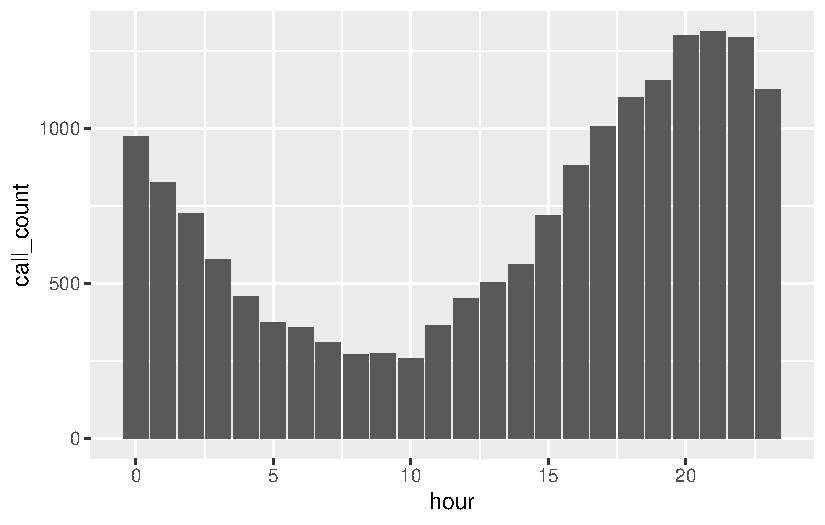
\includegraphics{hw2_files/figure-pdf/unnamed-chunk-12-1.pdf}

\subsubsection{Final write up}\label{final-write-up}

Q1. According to the table above, on average it takes 318.7497 seconds
for Wake County Fire to respond to incidents.

Q2. The response times do vary across all stations, station 29 has the
highest response time with a response time of 495.764 secs. Station 13
has the lowest response time with 223 secs.

Q3. Wake County Fire's response time has been been going down over time,
down to less than 300 secs after 2020. this may be due to an improvement
in technology, an increase in personnel could also be a factor in
reducing the response time.

Q4. Fire calls are most likely to occur from 21:00-23:00 hours.

Q5. 229047 calls are to Wake County Fire are recorded in this dataset,
and 17231 of those calls are actual fires.

Q6. The average response time for actual fires is 310.9837 secs, the
average response time for all incidents is 318.7497. Therefore, the
response time to actual fires averages was faster.

Q7.2 The average response time across all station varies. Station 23 had
the highest average response time with 586.3713 secs, station 3 had the
lowest average response time with 232.7666 secs.

Q7.3 Over time the average response time for wake county fire has been
going down, this decline may be due to improved infrastructures that
lead to better route options and a reduction in traffic.

Q7.4 Fire calls are most likely to occur for actual fires from
19:00-23:00, these fires could be happening because of faulty or
unattended equipment, technology, everyone charges their phones/tablets
before they go to sleep not caring about the dangers that may come with
such practices.

\subsection{Repository link:}\label{repository-link}

https://github.com/ashmandy/plan372-hw2.git



\end{document}
